If you use only the assignment's driver code, you'll implement rounding in Section~\ref{sec:encoding} but won't be able to test it until the end of Section~\ref{sec:addition}.
There \textit{is} a way that you can test your rounding code as soon as you've implemented it.
Many interactive debuggers allow you to change a variable's value at a breakpoint, and we shall take advantage of that feature.

\begin{description}
    \checkoffitem{Configure your debugger as necessary.}
    \checkoffitem{Set a breakpoint at the start of the \function{encode()} function. \\
        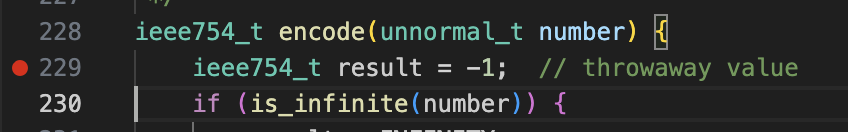
\includegraphics{rounding-images/setBreakpoint}
    }
    \checkoffitem{Launch \textit{floatlab} in the debugger, and use an input such as \texttt{\textbf{\textit{recode 1.1}}} \\
        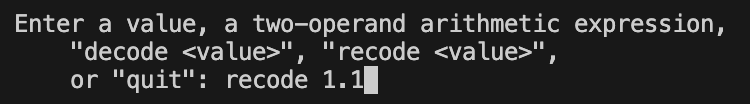
\includegraphics{rounding-images/enterTestValue}
    }
\end{description}

The driver code will parse the test value as an IEEE~754 single-precision value, so it will \textit{already} be rounded to fit in the available bits.
The trick is to re-introduce the bits that were rounded-off.

\begin{description}
    \checkoffitem{When the program reaches your breakpoint at the start of \function{encode()}, ``examine'' \lstinline{number.fraction}.}
    \checkoffitem{Instruct the debugger to change \lstinline{number.fraction}'s value.
        In VS~Code, this is done by right-clicking on the variable's name in the frame in which you're examining its value, and selecting ``Set Value''. \\
        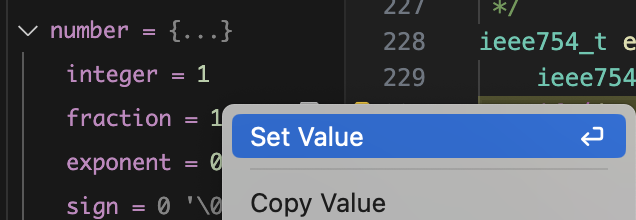
\includegraphics{rounding-images/selectSetValue}
    }
    \checkoffitem{Enter the 64-bit fraction for your test value in hexadecimal, such as \texttt{\textbf{\textit{recode 0x199999999999999A}}}
        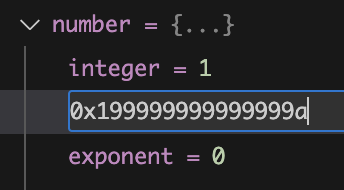
\includegraphics{rounding-images/newValueSet}
    }
    \checkoffitem{Instruct the debugger to continue. \\
        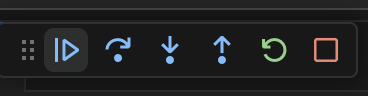
\includegraphics{rounding-images/selectContinue}
    }
    \checkoffitem{Compare the bit vector that your rounding code produced with the bit vector that it should have produced. \\
        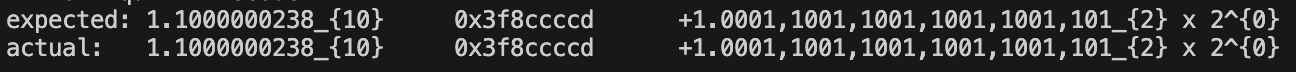
\includegraphics{rounding-images/results}
    }
\end{description}

\textit{Note: } Using this same technique to change \lstinline{number.exponent}, you can test your overflow-to-infinity and your underflow-to-zero code.

You may find these values useful for testing with the debugger:

\vspace{1cm}

\begin{tabular}[h]{ll}
    \textbf{Decimal Value}          & \textbf{64-bit fraction} \\
    \multicolumn{2}{c}{digit separators added for clarity; you won't be able to use them in the debugger} \\
    1.1                             & \texttt{0x1999'9999'9999'999A} \\
    1.3                             & \texttt{0x4CCC'CCCC'CCCC'CCCD} \\
    1.7                             & \texttt{0xB333'3333'3333'3333} \\
    1.9                             & \texttt{0xE666'6666'6666'6666} \\
    1.250'000'059'604'644'775'39    & \texttt{0x4000'0100'0000'0000} \\
    1.250'000'178'813'934'326'17    & \texttt{0x4000'0300'0000'0000}
\end{tabular}